\subsection{Design Simple Distributed System (Case Study Example 2)}

\begin{frame}[c]{ }
	\centering     
	
	\textcolor{offgreen}{ \large Previous video recap!}
\end{frame}

%%%%%%%%%%%%%%%%%%%%%%%%%%%%%%%%%%%%%%%%%%%%%%%%%%%%%%
\begin{frame}[plain,c]
	\frametitle{Case Study Example 1}
	\begin{figure}
		\centering
		


\tikzset{every picture/.style={line width=0.75pt}} %set default line width to 0.75pt        

\begin{tikzpicture}[scale=0.95,x=0.75pt,y=0.75pt,yscale=-1,xscale=1]
	%uncomment if require: \path (0,300); %set diagram left start at 0, and has height of 300
	
	%Shape: Rectangle [id:dp6258708726014198] 
	\draw  [color={rgb, 255:red, 74; green, 144; blue, 226 }  ,draw opacity=1 ][line width=1.5]  (60,151) -- (100,151) -- (100,189.67) -- (60,189.67) -- cycle ;

    %Node1
	%Shape: Frame [id:dp45199805556426453] 
	\draw  [line width=0.75,color=offwhite]  (445,57) -- (509,57) -- (509,97) -- (445,97) -- cycle(503,63) -- (451,63) -- (451,91) -- (503,91) -- cycle ;
	%Shape: Trapezoid [id:dp6365442083669953] 
	\draw  [line width=0.75,color=offwhite]  (435,127) -- (444,97) -- (510,97) -- (519,127) -- cycle ;
	%Shape: Trapezoid [id:dp7035229008077436] 
	\draw  [line width=0.75,color=offwhite]  (439,123) -- (446.5,98) -- (507.5,98) -- (515,123) -- cycle ;
	
    %Shape: Rectangle [id:dp4075005896181748] 
	\draw  [color={rgb, 255:red, 70; green, 155; blue, 36 }  ,draw opacity=1 ][line width=1.5]  (560.75,151) -- (610,151) -- (610,189) -- (560.75,189) -- cycle ;
	
    %output
    %Straight Lines [id:da7123818425757267] 
	\draw [color={rgb, 255:red, 128; green, 128; blue, 128 }  ,draw opacity=1 ]   (101,170) -- (128.88,169.84) ;
	\draw [shift={(130.88,169.83)}, rotate = 539.6800000000001] [color={rgb, 255:red, 128; green, 128; blue, 128 }  ,draw opacity=1 ][line width=0.75]    (10.93,-3.29) .. controls (6.95,-1.4) and (3.31,-0.3) .. (0,0) .. controls (3.31,0.3) and (6.95,1.4) .. (10.93,3.29)   ;
	
    %Shape: Rectangle [id:dp9860882909394741] 
	\draw  [color=offred  ,draw opacity=1 ][line width=0.75]  (230.75,119.63) -- (300.75,119.63) -- (300.75,149.63) -- (230.75,149.63) -- cycle ;
	%Shape: Rectangle [id:dp6809508870305205] 
	\draw  [color=offred  ,draw opacity=1 ][line width=0.75]  (229.75,189.63) -- (300.75,189.63) -- (300.75,219.63) -- (229.75,219.63) -- cycle ;
	
    %Curve Lines [id:da19696995243819926] 
	\draw [color={rgb, 255:red, 128; green, 128; blue, 128 }  ,draw opacity=1 ]   (169.75,190.63) .. controls (177.42,212.05) and (183.62,223.4) .. (228.38,219.75) ;
	\draw [shift={(229.75,219.63)}, rotate = 535.03] [color={rgb, 255:red, 128; green, 128; blue, 128 }  ,draw opacity=1 ][line width=0.75]    (10.93,-3.29) .. controls (6.95,-1.4) and (3.31,-0.3) .. (0,0) .. controls (3.31,0.3) and (6.95,1.4) .. (10.93,3.29)   ;
	%Curve Lines [id:da14087388365596432] 
	\draw [color={rgb, 255:red, 128; green, 128; blue, 128 }  ,draw opacity=1 ]   (169.75,149.63) .. controls (169.75,139.73) and (185.43,114.15) .. (229.41,119.46) ;
	\draw [shift={(230.75,119.63)}, rotate = 187.59] [color={rgb, 255:red, 128; green, 128; blue, 128 }  ,draw opacity=1 ][line width=0.75]    (10.93,-3.29) .. controls (6.95,-1.4) and (3.31,-0.3) .. (0,0) .. controls (3.31,0.3) and (6.95,1.4) .. (10.93,3.29)   ;
	%Curve Lines [id:da6655261202271237] 
	\draw [color={rgb, 255:red, 128; green, 128; blue, 128 }  ,draw opacity=1 ]   (300.75,119.63) .. controls (311.59,149.18) and (302.77,169.68) .. (336.19,170.64) ;
	\draw [shift={(337.75,170.67)}, rotate = 180.6] [color={rgb, 255:red, 128; green, 128; blue, 128 }  ,draw opacity=1 ][line width=0.75]    (10.93,-3.29) .. controls (6.95,-1.4) and (3.31,-0.3) .. (0,0) .. controls (3.31,0.3) and (6.95,1.4) .. (10.93,3.29)   ;
	%Curve Lines [id:da188937268210565] 
	\draw [color={rgb, 255:red, 128; green, 128; blue, 128 }  ,draw opacity=1 ]   (300.75,219.63) .. controls (310.55,191.21) and (304.74,171.12) .. (335.8,170.67) ;
	\draw [shift={(337.75,170.67)}, rotate = 180.63] [color={rgb, 255:red, 128; green, 128; blue, 128 }  ,draw opacity=1 ][line width=0.75]    (10.93,-3.29) .. controls (6.95,-1.4) and (3.31,-0.3) .. (0,0) .. controls (3.31,0.3) and (6.95,1.4) .. (10.93,3.29)   ;
	
    %Shape: Rectangle [id:dp795964462639149] 
	\draw  [color=offyellow  ,draw opacity=1 ] (131,151) -- (201,151) -- (201,190) -- (131,190) -- cycle ;

	%Shape: Frame [id:dp7417485861438164] 
	\draw  [line width=0.75,color=offwhite]  (443,212) -- (507,212) -- (507,252) -- (443,252) -- cycle(501,218) -- (449,218) -- (449,246) -- (501,246) -- cycle ;
	%Shape: Trapezoid [id:dp7528630303015812] 
	\draw  [line width=0.75,color=offwhite]  (433,282) -- (442,252) -- (508,252) -- (517,282) -- cycle ;
	%Shape: Trapezoid [id:dp8885841590443699] 
	\draw  [line width=0.75,color=offwhite]  (437,278) -- (444.5,253) -- (505.5,253) -- (513,278) -- cycle ;

    %????
	%Shape: Rectangle [id:dp6221340422393318] 
	\draw  [color=offpurple,line width=0.75] (340,151) -- (389.75,151) -- (389.75,189.67) -- (340,189.67) -- cycle ;

	%Curve Lines [id:da17799352827092774] 
	\draw [color={rgb, 255:red, 128; green, 128; blue, 128 }  ,draw opacity=1 ]   (390,170.17) .. controls (415.99,126.11) and (392.72,97.25) .. (442.47,97) ;
	\draw [shift={(444,97)}, rotate = 180.37] [color={rgb, 255:red, 128; green, 128; blue, 128 }  ,draw opacity=1 ][line width=0.75]    (10.93,-3.29) .. controls (6.95,-1.4) and (3.31,-0.3) .. (0,0) .. controls (3.31,0.3) and (6.95,1.4) .. (10.93,3.29)   ;
	
    %Curve Lines [id:da9685723605797839] 
	\draw [color={rgb, 255:red, 128; green, 128; blue, 128 }  ,draw opacity=1 ]   (390,170.17) .. controls (415.86,237.64) and (399.75,251.26) .. (440.12,251.98) ;
	\draw [shift={(442,252)}, rotate = 180.45] [color={rgb, 255:red, 128; green, 128; blue, 128 }  ,draw opacity=1 ][line width=0.75]    (10.93,-3.29) .. controls (6.95,-1.4) and (3.31,-0.3) .. (0,0) .. controls (3.31,0.3) and (6.95,1.4) .. (10.93,3.29)   ;
	
    %Curve Lines [id:da43813209116711305] 
	\draw [color={rgb, 255:red, 128; green, 128; blue, 128 }  ,draw opacity=1 ]   (510,97) .. controls (541.27,124.58) and (518.46,169.62) .. (557,172.88) ;
	\draw [shift={(558,173)}, rotate = 182.66] [color={rgb, 255:red, 128; green, 128; blue, 128 }  ,draw opacity=1 ][line width=0.75]    (10.93,-3.29) .. controls (6.95,-1.4) and (3.31,-0.3) .. (0,0) .. controls (3.31,0.3) and (6.95,1.4) .. (10.93,3.29)   ;
	
    %Curve Lines [id:da5479643719173531] 
	\draw [color={rgb, 255:red, 128; green, 128; blue, 128 }  ,draw opacity=1 ]   (508,252) .. controls (536.96,209.1) and (511.27,191.36) .. (557,173.54) ;
	\draw [shift={(558,173)}, rotate = 520.2] [color={rgb, 255:red, 128; green, 128; blue, 128 }  ,draw opacity=1 ][line width=0.75]    (10.93,-3.29) .. controls (6.95,-1.4) and (3.31,-0.3) .. (0,0) .. controls (3.31,0.3) and (6.95,1.4) .. (10.93,3.29)   ;
	

	% Text Node
	\draw (65,208) node [anchor=north west][inner sep=0.75pt]  [font=\footnotesize,color={rgb, 255:red, 74; green, 144; blue, 226 }  ,opacity=1 ]  {Input};
	% Text Node
	\draw (65,164) node [anchor=north west][inner sep=0.75pt]  [font=\scriptsize,color={rgb, 255:red, 74; green, 144; blue, 226 }  ,opacity=1 ]  {Hello};
	% Text Node
	\draw (454,131) node [anchor=north west][inner sep=0.75pt]  [font=\footnotesize,color=offwhite]  {Node 1};
	% Text Node
	\draw (564,167) node [anchor=north west][inner sep=0.75pt]  [font=\scriptsize,color={rgb, 255:red, 70; green, 155; blue, 36 }  ,opacity=1 ]  {HELLO};
	% Text Node
	\draw (564,208) node [anchor=north west][inner sep=0.75pt]  [font=\footnotesize,color={rgb, 255:red, 70; green, 155; blue, 36 }  ,opacity=1 ]  {Output};
	% Text Node
	\draw (141,164) node [anchor=north west][inner sep=0.75pt]  [font=\scriptsize,color=offyellow  ,opacity=1 ]  {File Split};
	% Text Node
	\draw (248,131) node [anchor=north west][inner sep=0.75pt]  [font=\scriptsize,color=offred  ,opacity=1 ]  {Split-1};
	% Text Node
	\draw (248,200) node [anchor=north west][inner sep=0.75pt]  [font=\scriptsize,color=offred  ,opacity=1 ]  {Split-2};
	% Text Node
	\draw (454,286) node [anchor=north west][inner sep=0.75pt]  [font=\footnotesize,color=offwhite]  {Node 2};
	% Text Node
	\draw (346,165) node [anchor=north west][inner sep=0.75pt]  [font=\scriptsize,color=offpurple]  {$S_x$ \% n };
    \draw (340,210) node [anchor=north west][inner sep=0.75pt]  [font=\scriptsize,color=offpurple]  {Mgmt Box};

    
	
\end{tikzpicture}

		\caption{Convert text to upper text, for example, The -> THE } \label{fig:DS3}
	\end{figure}
	
\end{frame}
%%%%%%%%%%%%%%%%%%%%%%%%%%%%%%%%%%%%%%%%%%%%%%%%%%%%%%
\begin{frame}[plain,c]
	\frametitle{Case Study Example 1}
	\begin{figure}
		\centering
		


\tikzset{every picture/.style={line width=0.75pt}} %set default line width to 0.75pt        

\begin{tikzpicture}[scale=0.95,x=0.75pt,y=0.75pt,yscale=-1,xscale=1]
	%uncomment if require: \path (0,300); %set diagram left start at 0, and has height of 300
	
	%Shape: Rectangle [id:dp6258708726014198] 
	\draw  [color={rgb, 255:red, 74; green, 144; blue, 226 }  ,draw opacity=1 ][line width=1.5]  (60,151) -- (100,151) -- (100,189.67) -- (60,189.67) -- cycle ;

    %Node1
	%Shape: Frame [id:dp45199805556426453] 
	\draw  [line width=0.75,color=offwhite]  (445,57) -- (509,57) -- (509,97) -- (445,97) -- cycle(503,63) -- (451,63) -- (451,91) -- (503,91) -- cycle ;
	%Shape: Trapezoid [id:dp6365442083669953] 
	\draw  [line width=0.75,color=offwhite]  (435,127) -- (444,97) -- (510,97) -- (519,127) -- cycle ;
	%Shape: Trapezoid [id:dp7035229008077436] 
	\draw  [line width=0.75,color=offwhite]  (439,123) -- (446.5,98) -- (507.5,98) -- (515,123) -- cycle ;
	
    %Shape: Rectangle [id:dp4075005896181748] 
	\draw  [color={rgb, 255:red, 70; green, 155; blue, 36 }  ,draw opacity=1 ][line width=1.5]  (560.75,151) -- (610,151) -- (610,189) -- (560.75,189) -- cycle ;
	
    %output
    %Straight Lines [id:da7123818425757267] 
	\draw [color={rgb, 255:red, 128; green, 128; blue, 128 }  ,draw opacity=1 ]   (101,170) -- (128.88,169.84) ;
	\draw [shift={(130.88,169.83)}, rotate = 539.6800000000001] [color={rgb, 255:red, 128; green, 128; blue, 128 }  ,draw opacity=1 ][line width=0.75]    (10.93,-3.29) .. controls (6.95,-1.4) and (3.31,-0.3) .. (0,0) .. controls (3.31,0.3) and (6.95,1.4) .. (10.93,3.29)   ;
	
    %Shape: Rectangle [id:dp9860882909394741] 
	\draw  [color=offred  ,draw opacity=1 ][line width=0.75]  (230.75,119.63) -- (300.75,119.63) -- (300.75,149.63) -- (230.75,149.63) -- cycle ;
	%Shape: Rectangle [id:dp6809508870305205] 
	\draw  [color=offred  ,draw opacity=1 ][line width=0.75]  (229.75,189.63) -- (300.75,189.63) -- (300.75,219.63) -- (229.75,219.63) -- cycle ;
	
    %Curve Lines [id:da19696995243819926] 
	\draw [color={rgb, 255:red, 128; green, 128; blue, 128 }  ,draw opacity=1 ]   (169.75,190.63) .. controls (177.42,212.05) and (183.62,223.4) .. (228.38,219.75) ;
	\draw [shift={(229.75,219.63)}, rotate = 535.03] [color={rgb, 255:red, 128; green, 128; blue, 128 }  ,draw opacity=1 ][line width=0.75]    (10.93,-3.29) .. controls (6.95,-1.4) and (3.31,-0.3) .. (0,0) .. controls (3.31,0.3) and (6.95,1.4) .. (10.93,3.29)   ;
	%Curve Lines [id:da14087388365596432] 
	\draw [color={rgb, 255:red, 128; green, 128; blue, 128 }  ,draw opacity=1 ]   (169.75,149.63) .. controls (169.75,139.73) and (185.43,114.15) .. (229.41,119.46) ;
	\draw [shift={(230.75,119.63)}, rotate = 187.59] [color={rgb, 255:red, 128; green, 128; blue, 128 }  ,draw opacity=1 ][line width=0.75]    (10.93,-3.29) .. controls (6.95,-1.4) and (3.31,-0.3) .. (0,0) .. controls (3.31,0.3) and (6.95,1.4) .. (10.93,3.29)   ;
	%Curve Lines [id:da6655261202271237] 
	\draw [color={rgb, 255:red, 128; green, 128; blue, 128 }  ,draw opacity=1 ]   (300.75,119.63) .. controls (311.59,149.18) and (302.77,169.68) .. (336.19,170.64) ;
	\draw [shift={(337.75,170.67)}, rotate = 180.6] [color={rgb, 255:red, 128; green, 128; blue, 128 }  ,draw opacity=1 ][line width=0.75]    (10.93,-3.29) .. controls (6.95,-1.4) and (3.31,-0.3) .. (0,0) .. controls (3.31,0.3) and (6.95,1.4) .. (10.93,3.29)   ;
	%Curve Lines [id:da188937268210565] 
	\draw [color={rgb, 255:red, 128; green, 128; blue, 128 }  ,draw opacity=1 ]   (300.75,219.63) .. controls (310.55,191.21) and (304.74,171.12) .. (335.8,170.67) ;
	\draw [shift={(337.75,170.67)}, rotate = 180.63] [color={rgb, 255:red, 128; green, 128; blue, 128 }  ,draw opacity=1 ][line width=0.75]    (10.93,-3.29) .. controls (6.95,-1.4) and (3.31,-0.3) .. (0,0) .. controls (3.31,0.3) and (6.95,1.4) .. (10.93,3.29)   ;
	
    %Shape: Rectangle [id:dp795964462639149] 
	\draw  [color=offyellow  ,draw opacity=1 ] (131,151) -- (201,151) -- (201,190) -- (131,190) -- cycle ;

	%Shape: Frame [id:dp7417485861438164] 
	\draw  [line width=0.75,color=offwhite]  (443,212) -- (507,212) -- (507,252) -- (443,252) -- cycle(501,218) -- (449,218) -- (449,246) -- (501,246) -- cycle ;
	%Shape: Trapezoid [id:dp7528630303015812] 
	\draw  [line width=0.75,color=offwhite]  (433,282) -- (442,252) -- (508,252) -- (517,282) -- cycle ;
	%Shape: Trapezoid [id:dp8885841590443699] 
	\draw  [line width=0.75,color=offwhite]  (437,278) -- (444.5,253) -- (505.5,253) -- (513,278) -- cycle ;

    %????
	%Shape: Rectangle [id:dp6221340422393318] 
	\draw  [color=offpurple,line width=0.75] (340,151) -- (389.75,151) -- (389.75,189.67) -- (340,189.67) -- cycle ;

	%Curve Lines [id:da17799352827092774] 
	\draw [color={rgb, 255:red, 128; green, 128; blue, 128 }  ,draw opacity=1 ]   (390,170.17) .. controls (415.99,126.11) and (392.72,97.25) .. (442.47,97) ;
	\draw [shift={(444,97)}, rotate = 180.37] [color={rgb, 255:red, 128; green, 128; blue, 128 }  ,draw opacity=1 ][line width=0.75]    (10.93,-3.29) .. controls (6.95,-1.4) and (3.31,-0.3) .. (0,0) .. controls (3.31,0.3) and (6.95,1.4) .. (10.93,3.29)   ;
	
    %Curve Lines [id:da9685723605797839] 
	\draw [color={rgb, 255:red, 128; green, 128; blue, 128 }  ,draw opacity=1 ]   (390,170.17) .. controls (415.86,237.64) and (399.75,251.26) .. (440.12,251.98) ;
	\draw [shift={(442,252)}, rotate = 180.45] [color={rgb, 255:red, 128; green, 128; blue, 128 }  ,draw opacity=1 ][line width=0.75]    (10.93,-3.29) .. controls (6.95,-1.4) and (3.31,-0.3) .. (0,0) .. controls (3.31,0.3) and (6.95,1.4) .. (10.93,3.29)   ;
	
    %Curve Lines [id:da43813209116711305] 
	\draw [color={rgb, 255:red, 128; green, 128; blue, 128 }  ,draw opacity=1 ]   (510,97) .. controls (541.27,124.58) and (518.46,169.62) .. (557,172.88) ;
	\draw [shift={(558,173)}, rotate = 182.66] [color={rgb, 255:red, 128; green, 128; blue, 128 }  ,draw opacity=1 ][line width=0.75]    (10.93,-3.29) .. controls (6.95,-1.4) and (3.31,-0.3) .. (0,0) .. controls (3.31,0.3) and (6.95,1.4) .. (10.93,3.29)   ;
	
    %Curve Lines [id:da5479643719173531] 
	\draw [color={rgb, 255:red, 128; green, 128; blue, 128 }  ,draw opacity=1 ]   (508,252) .. controls (536.96,209.1) and (511.27,191.36) .. (557,173.54) ;
	\draw [shift={(558,173)}, rotate = 520.2] [color={rgb, 255:red, 128; green, 128; blue, 128 }  ,draw opacity=1 ][line width=0.75]    (10.93,-3.29) .. controls (6.95,-1.4) and (3.31,-0.3) .. (0,0) .. controls (3.31,0.3) and (6.95,1.4) .. (10.93,3.29)   ;

    %Shape: Cloud [id:dp9284795120380853] 
    \draw  [color={rgb, 255:red, 80; green, 227; blue, 194 }  ,draw opacity=1 ][dash pattern={on 1.69pt off 2.76pt}][line width=1.5]  (313.65,190.77) .. controls (314.97,206.06) and (308.48,220.94) .. (296.96,229.1) .. controls (285.42,237.25) and (270.87,237.25) .. (259.47,229.09) .. controls (255.04,237.81) and (247.28,243.67) .. (238.53,244.91) .. controls (229.77,246.14) and (221.06,242.6) .. (215.02,235.35) .. controls (211.23,243.26) and (204.14,248.43) .. (196.27,249.02) .. controls (188.39,249.6) and (180.84,245.52) .. (176.3,238.22) .. controls (169.66,246.52) and (159.43,249.77) .. (150.03,246.56) .. controls (140.63,243.35) and (133.76,234.26) .. (132.38,223.21) .. controls (124.67,220.53) and (118.39,214.17) .. (115.15,205.77) .. controls (111.92,197.36) and (112.05,187.74) .. (115.52,179.39) .. controls (108.22,167.77) and (106.93,152.57) .. (112.13,139.47) .. controls (117.32,126.36) and (128.22,117.31) .. (140.75,115.7) .. controls (141.25,103.25) and (147.63,92.02) .. (157.43,86.35) .. controls (167.23,80.68) and (178.92,81.44) .. (187.99,88.34) .. controls (192.44,73.56) and (203.94,62.96) .. (217.53,61.12) .. controls (231.11,59.28) and (244.34,66.53) .. (251.49,79.73) .. controls (261.01,73.66) and (272.23,72.19) .. (282.63,75.66) .. controls (293.03,79.13) and (301.73,87.25) .. (306.77,98.18) .. controls (316.32,97.23) and (325.32,103.14) .. (329.31,112.98) .. controls (333.3,122.82) and (331.43,134.49) .. (324.63,142.2) .. controls (332.92,148.17) and (336.87,159.58) .. (334.42,170.5) .. controls (331.97,181.41) and (323.68,189.36) .. (313.87,190.18) ; \draw  [color={rgb, 255:red, 80; green, 227; blue, 194 }  ,draw opacity=1 ][dash pattern={on 1.69pt off 2.76pt}][line width=1.5]  (324.62,142.21) .. controls (320.71,139.39) and (316.13,138.02) .. (311.49,138.28)(306.77,98.18) .. controls (304.77,98.38) and (302.8,98.88) .. (300.92,99.66)(251.49,79.73) .. controls (252.82,82.16) and (253.9,84.76) .. (254.73,87.46)(187.99,88.34) .. controls (187.17,91.03) and (186.61,93.82) .. (186.31,96.64)(140.75,115.7) .. controls (140.22,128.95) and (146.42,141.31) .. (156.71,147.46)(115.52,179.39) .. controls (117.37,174.93) and (120.09,171.01) .. (123.48,167.94)(132.38,223.21) .. controls (132.15,221.38) and (132.08,219.52) .. (132.17,217.67)(176.3,238.22) .. controls (177.96,236.15) and (179.34,233.82) .. (180.41,231.31)(215.02,235.35) .. controls (215.93,233.45) and (216.63,231.43) .. (217.1,229.34)(259.47,229.09) .. controls (257.06,227.36) and (254.84,225.3) .. (252.87,222.97)(313.65,190.77) .. controls (313.47,188.66) and (313.15,186.57) .. (312.68,184.53) ;
    
    %Rounded Rect [id:dp4710145421837679] 
    \draw  [color={rgb, 255:red, 196; green, 158; blue, 126 }  ,draw opacity=1 ][dash pattern={on 5.63pt off 4.5pt}][line width=1.5]  (513.82,33.19) .. controls (530.18,33.2) and (543.44,46.47) .. (543.43,62.83) -- (543.32,278.58) .. controls (543.31,294.94) and (530.04,308.2) .. (513.67,308.19) -- (424.78,308.14) .. controls (408.42,308.13) and (395.16,294.86) .. (395.17,278.5) -- (395.28,62.76) .. controls (395.29,46.39) and (408.56,33.13) .. (424.93,33.14) -- cycle ;

    %Straight Lines [id:da03293914629554606] 


    %Straight Lines [id:da03293914629554606] 
    \draw [color=offpurple  ][line width=1.5]  [dash pattern={on 1.69pt off 2.76pt}]  (361.25,294.17) -- (361.25,202.17) ;
    \draw [shift={(361.25,199.17)}, rotate = 450] [color=offpurple  ][line width=1.5]    (14.21,-4.28) .. controls (9.04,-1.82) and (4.3,-0.39) .. (0,0) .. controls (4.3,0.39) and (9.04,1.82) .. (14.21,4.28)   ;




	% Text Node
	\draw (65,208) node [anchor=north west][inner sep=0.75pt]  [font=\footnotesize,color={rgb, 255:red, 74; green, 144; blue, 226 }  ,opacity=1 ]  {Input};
	% Text Node
	\draw (65,164) node [anchor=north west][inner sep=0.75pt]  [font=\scriptsize,color={rgb, 255:red, 74; green, 144; blue, 226 }  ,opacity=1 ]  {Hello};
	% Text Node
	\draw (454,131) node [anchor=north west][inner sep=0.75pt]  [font=\footnotesize,color=offwhite]  {Node 1};
	% Text Node
	\draw (564,167) node [anchor=north west][inner sep=0.75pt]  [font=\scriptsize,color={rgb, 255:red, 70; green, 155; blue, 36 }  ,opacity=1 ]  {HELLO};
	% Text Node
	\draw (564,208) node [anchor=north west][inner sep=0.75pt]  [font=\footnotesize,color={rgb, 255:red, 70; green, 155; blue, 36 }  ,opacity=1 ]  {Output};
	% Text Node
	\draw (141,164) node [anchor=north west][inner sep=0.75pt]  [font=\scriptsize,color=offyellow  ,opacity=1 ]  {File Split};
	% Text Node
	\draw (248,131) node [anchor=north west][inner sep=0.75pt]  [font=\scriptsize,color=offred  ,opacity=1 ]  {Split-1};
	% Text Node
	\draw (248,200) node [anchor=north west][inner sep=0.75pt]  [font=\scriptsize,color=offred  ,opacity=1 ]  {Split-2};
	% Text Node
	\draw (454,286) node [anchor=north west][inner sep=0.75pt]  [font=\footnotesize,color=offwhite]  {Node 2};
	% Text Node
	\draw (354,165) node [anchor=north west][inner sep=0.75pt]  [font=\scriptsize,color=offpurple]  {???};
    \draw (340,313) node [anchor=north west][inner sep=0.75pt]  [font=\scriptsize,color=offpurple]  {Mgmt Box};

    \draw (166,313) node [anchor=north west][inner sep=0.75pt]  [font=\footnotesize,color={rgb, 255:red, 80; green, 227; blue, 194 }  ,opacity=1 ] [align=left] {File System Box};

	
    % Text Node
    \draw (418,313) node [anchor=north west][inner sep=0.75pt]  [font=\footnotesize,color={rgb, 255:red, 196; green, 158; blue, 126 }  ,opacity=1 ] [align=left] {Processing Box};



\end{tikzpicture}

	\end{figure}
	
\end{frame}
%%%%%%%%%%%%%%%%%%%%%%%%%%%%%%%%%%%%%%%%%%%%%%%%%%%%%%
\begin{frame}
	\frametitle{Case Study Example 2}
	\begin{itemize}  [<+->]
		\item Assume we have a file contains \textbf{\underline{1TB}} of text lines, and we need to calculate the word count across the document, for example, \textcolor{offyellow}{The cat came back the very next day} -> \textcolor{brown}{(the, 2), (cat,1), (came,1), (back, 1), (very, 1), (next, 1), (day, 1)}.

		\item One of the distributed architecture solutions for this problem is to use \textcolor{offyellow}{\textit{map-reduce}}.
	\end{itemize}
\end{frame}

%%%%%%%%%%%%%%%%%%%%%%%%%%%%%%%%%%%%%%%%%%%%%%%%%%%%%%
\begin{frame}
	\frametitle{The basic idea of MapReduce}
	\begin{itemize}  [<+->]
		\item Assume we need to launch a high-throughput bulk-production sandwich shop. 
		\item This sandwich has a lot of raw ingredients, and our target is to produce the sandwich as quickly as possible.
		\item To make the production very quickly we need to distribute the tasks between the  \textcolor{offyellow}{\textit{workers}}.				
	\end{itemize}
	\footnotetext[1]{This example taken from  \href{https://reberhardt.com/cs110/summer-2018/lecture-notes/lecture-14/}{https://reberhardt.com/cs110/summer-2018/lecture-notes/lecture-14/}	} 
\end{frame}
%%%%%%%%%%%%%%%%%%%%%%%%%%%%%%%%%%%%%%%%%%%%%%%%%%%%%%
\begin{frame}
	\frametitle{The basic idea of MapReduce}
	We break this into three stages
	\begin{itemize}  [<+->]
		\item Map.
		\item Shuffle/Group (Mapper Intermediates).
		\item Reduce			
	\end{itemize}
	\footnotetext[1]{This example taken from  \href{https://reberhardt.com/cs110/summer-2018/lecture-notes/lecture-14/}{https://reberhardt.com/cs110/summer-2018/lecture-notes/lecture-14/}	} 
\end{frame}
%%%%%%%%%%%%%%%%%%%%%%%%%%%%%%%%%%%%%%%%%%%%%%%%%%%%%%
\begin{frame}
	\frametitle{Map}
	We distribute our raw ingredients amongst the workers.
	\begin{figure}
		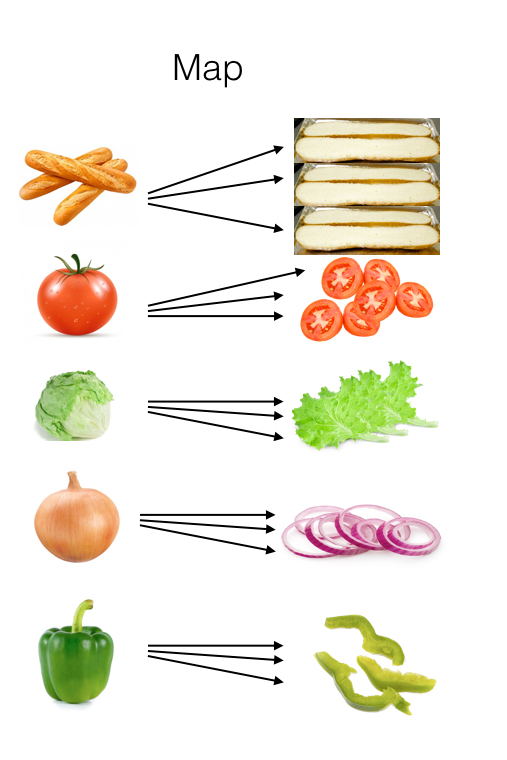
\includegraphics[width=.5\textwidth,height=.7\textheight]{./Figures/chapter-02/map-reduce-map-side.jpeg}
	\end{figure}			
	\footnotetext[1]{{\tiny This example taken from  \href{https://reberhardt.com/cs110/summer-2018/lecture-notes/lecture-14/}{https://reberhardt.com/cs110/summer-2018/lecture-notes/lecture-14/}	} }
\end{frame}
%%%%%%%%%%%%%%%%%%%%%%%%%%%%%%%%%%%%%%%%%%%%%%%%%%%%%%
\begin{frame}
	\frametitle{Shuffle/Group}
	We will organise and group the processed ingredients into piles, so that making a sandwich becomes easy.
		\begin{figure}
		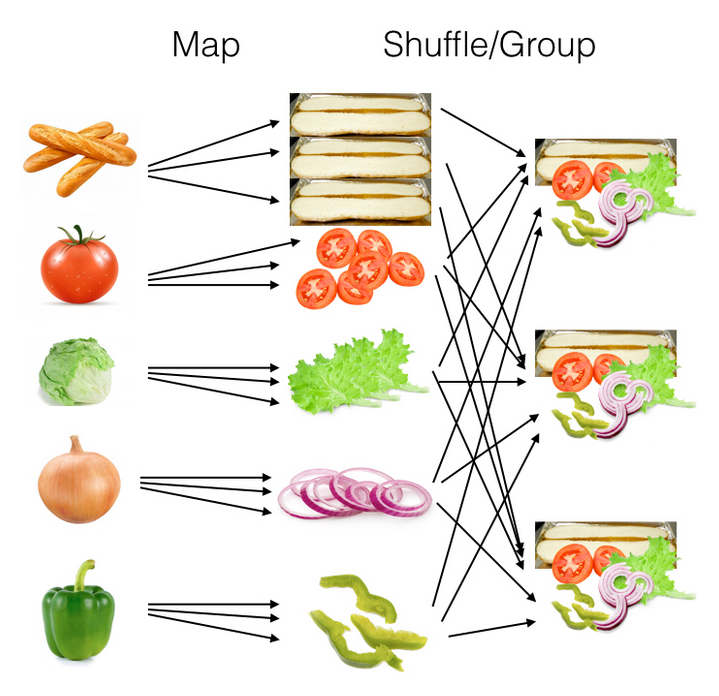
\includegraphics[width=.7\textwidth,height=.64\textheight]{./Figures/chapter-02/map-reduce-shuffle.png}
	\end{figure}			
	\footnotetext[1]{{\tiny This example taken from  \href{https://reberhardt.com/cs110/summer-2018/lecture-notes/lecture-14/}{https://reberhardt.com/cs110/summer-2018/lecture-notes/lecture-14/}	}} 
\end{frame}
%%%%%%%%%%%%%%%%%%%%%%%%%%%%%%%%%%%%%%%%%%%%%%%%%%%%%%
\begin{frame}
	\frametitle{Reduce}
	we’ll combine the ingredients into a sandwich
	\begin{figure}
		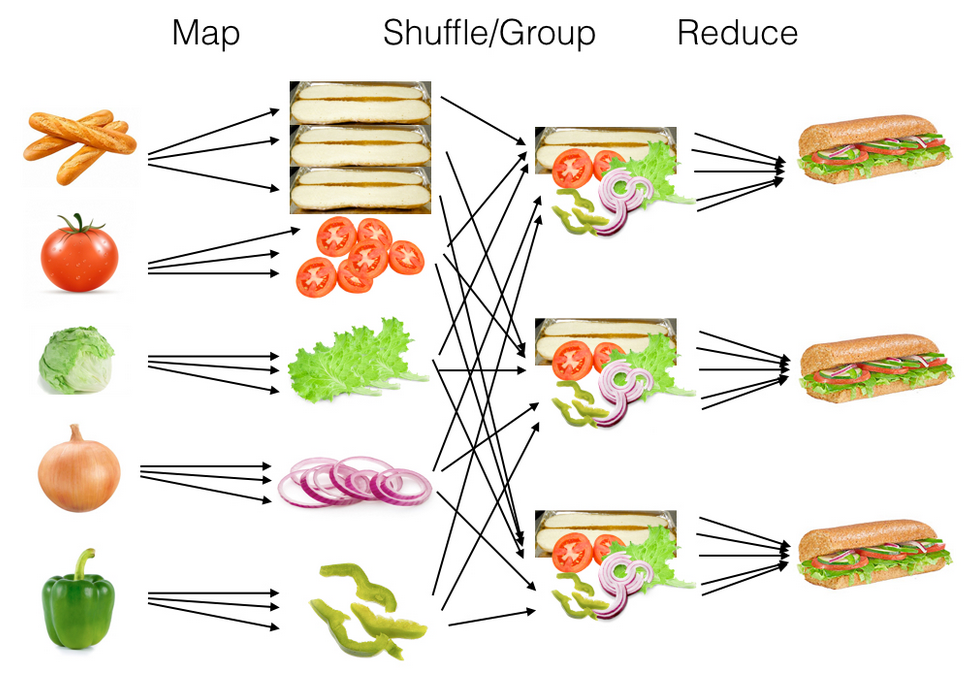
\includegraphics[width=.96\textwidth,height=.7\textheight]{./Figures/chapter-02/map-reduce-reduce-side.png}
	\end{figure}			
	\footnotetext[1]{ {\tiny This example taken from  \href{https://reberhardt.com/cs110/summer-2018/lecture-notes/lecture-14/}{https://reberhardt.com/cs110/summer-2018/lecture-notes/lecture-14/}	}} 
\end{frame}


%%%%%%%%%%%%%%%%%%%%%%%%%%%%%%%%%%%%%%%%%%%%%%%%%%%%%%
\begin{frame}[plain,c]
	\frametitle{Case Study Example 2}
	\begin{figure}
		\centering
		


\tikzset{every picture/.style={line width=0.75pt}} %set default line width to 0.75pt        

\begin{tikzpicture}[x=0.65pt,y=0.65pt,yscale=-1,xscale=1]
	%uncomment if require: \path (0,221); %set diagram left start at 0, and has height of 221
	
	
	%Shape: Rectangle [id:dp3221278753230701] 
	\draw [color=offred]  (2,60) -- (111,60) -- (111,90) -- (2,90) -- cycle ;
	%Shape: Rectangle [id:dp1271633566749788] 
	\draw [color=offred]  (2,140) -- (111,140) -- (111,170) -- (2,170) -- cycle ;
	%Curve Lines [id:da7576806433421945] 
	\draw  [line width=0.75,color=offwhite]  (112.42,59) .. controls (125,77.7) and (100.24,107.85) .. (128.62,109.05) ;

	%Curve Lines [id:da7014275949258858] 
	\draw [line width=0.75,color=offwhite]   (112,161.08) .. controls (125,137.56) and (97.32,110.2) .. (128.44,109.12) ;
	\draw [line width=0.75,color=offwhite] [shift={(130.42,109.08)}, rotate = 180] [color=offwhite  ][line width=0.75]    (10.93,-3.29) .. controls (6.95,-1.4) and (3.31,-0.3) .. (0,0) .. controls (3.31,0.3) and (6.95,1.4) .. (10.93,3.29)   ;
	%Rounded Rect [id:dp8577127496471914] 
	\draw   [color=offpurple] (131,103.47) .. controls (131,101.05) and (132.96,99.08) .. (135.38,99.08) -- (166.03,99.08) .. controls (168.45,99.08) and (170.42,101.05) .. (170.42,103.47) -- (170.42,116.62) .. controls (170.42,119.04) and (168.45,121) .. (166.03,121) -- (135.38,121) .. controls (132.96,121) and (131,119.04) .. (131,116.62) -- cycle ;
	%Rounded Rect [id:dp30434364847793793] 
	%%SPLIT 1
	\draw   [color={rgb, 255:red, 74; green, 144; blue, 226 }] 	(200,60) -- (250,60) -- (250,90) -- (200,90) -- cycle ;
	%Rounded Rect [id:dp4147495296848157] 
	%%SPLIT2
	
	\draw    [color={rgb, 255:red, 74; green, 144; blue, 226 }]  	(200,140) -- (250,140) -- (250,170) -- (200,170) -- cycle ;
	
	
	%Shape: Parallelogram [id:dp48792900018844987] 
	%%MAP
	\draw  [color=offyellow] (290,55.58) -- (323,55.58) -- (309,84) -- (277,84) -- cycle ;
	%Shape: Parallelogram [id:dp15766656313302363] 
	\draw [color=offyellow]  (290,140) -- (323,140) -- (309,166) -- (277,166) -- cycle ;
	
	%Straight Lines [id:da44147302793163634] 
	\draw  [line width=0.75,color=offwhite]  (251,70.79) -- (276,70.6) ;
	\draw  [line width=0.75,color=offwhite][shift={(280,70.58)}, rotate = 539.53] [color=offwhite  ][line width=0.75]    (10.93,-3.29) .. controls (6.95,-1.4) and (3.31,-0.3) .. (0,0) .. controls (3.31,0.3) and (6.95,1.4) .. (10.93,3.29)   ;
	
	
	%Straight Lines [id:da9443785238686285] 
	\draw  [line width=0.75,color=offwhite]  (251,151.79) -- (276,151.6) ;
	\draw [line width=0.75,color=offwhite] [shift={(278.42,151.58)}, rotate = 539.56] [color=offwhite  ][line width=0.75]    (10.93,-3.29) .. controls (6.95,-1.4) and (3.31,-0.3) .. (0,0) .. controls (3.31,0.3) and (6.95,1.4) .. (10.93,3.29)   ;
	%Shape: Rectangle [id:dp016273691107661636] 
	\draw [color={rgb, 255:red, 70; green, 155; blue, 36 }]  (342,47.58) -- (390,47.58) -- (390,106.58) -- (343,106.58) -- cycle ;
	%Straight Lines [id:da747872157663686] 
	\draw  [line width=0.75,color=offwhite]  (317,70) -- (338,70) ;
	\draw  [line width=0.75,color=offwhite] [shift={(340,70.58)}, rotate = 539.53] [color=offwhite  ][line width=0.75]    (10.93,-3.29) .. controls (6.95,-1.4) and (3.31,-0.3) .. (0,0) .. controls (3.31,0.3) and (6.95,1.4) .. (10.93,3.29)   ;
	%Straight Lines [id:da29503611504052674] 
	\draw  [line width=0.75,color=offwhite]  (317,156) -- (338,156) ;
\draw [line width=0.75,color=offwhite] [shift={(340.42,156.58)}, rotate = 539.53] [color=offwhite  ][line width=0.75]    (10.93,-3.29) .. controls (6.95,-1.4) and (3.31,-0.3) .. (0,0) .. controls (3.31,0.3) and (6.95,1.4) .. (10.93,3.29)   ;
	%Shape: Rectangle [id:dp4945355441436542] 
	%output
	\draw [color={rgb, 255:red, 70; green, 155; blue, 36 }]  (342,121) -- (390,121) -- (390,182.58) -- (343,182.58) -- cycle ;
	%Shape: Rectangle [id:dp7486542282421536] 
	%% outer box
	\draw   (188,20.58) -- (398.42,20.58) -- (398.42,110.58) -- (188,110.58) -- cycle ;
	%Shape: Rectangle [id:dp06285129437676396] 
	%%outerbox
	\draw   (188,110.58) -- (398.42,110.58) -- (398.42,200.58) -- (188,200.58) -- cycle ;
	%Rounded Rect [id:dp7025642442655686] 
	\draw   (414.42,98.18) .. controls (414.42,94.54) and (417.37,91.58) .. (421.02,91.58) -- (444.82,91.58) .. controls (448.46,91.58) and (451.42,94.54) .. (451.42,98.18) -- (451.42,117.98) .. controls (451.42,121.63) and (448.46,124.58) .. (444.82,124.58) -- (421.02,124.58) .. controls (417.37,124.58) and (414.42,121.63) .. (414.42,117.98) -- cycle ;
	%Shape: Rectangle [id:dp7889635565295128] 
	%% outer box
	\draw   (468.42,19.58) -- (670.42,19.58) -- (670.42,110.58) -- (468.42,110.58) -- cycle ;
	%Shape: Rectangle [id:dp8905165615601378] 
	%% outer box
	\draw   (468.42,110.58) -- (670.42,110.58) -- (670.42,200.58) -- (468.42,200.58) -- cycle ;
	%Shape: Rectangle [id:dp38010158785945036] 
	%input
	\draw [color={rgb, 255:red, 74; green, 144; blue, 226 } ]  (471,39.58) -- (523.42,39.58) -- (523.42,100.58) -- (471,100.58) -- cycle ;
	%Shape: Rectangle [id:dp7112194600890194] 
	%input
	\draw  [color={rgb, 255:red, 74; green, 144; blue, 226 } ] (471,127) -- (528.42,127) -- (528.42,187.58) -- (471,187.58) -- cycle ;
	
	%Shape: Parallelogram [id:dp8560234333811613] 
	\draw [color=offpink]  (555,53.58) -- (593,53.58) -- (580,82) -- (544,82) -- cycle ;
	%Shape: Parallelogram [id:dp03185670047818545] 
	\draw [color=offpink]  (555,132.58) -- (593,132.58) -- (580,161) -- (544,161) -- cycle ;
	
	
	%Shape: Rectangle [id:dp7083827174523002] 
	%output
	\draw [color={rgb, 255:red, 70; green, 155; blue, 36 }]  (610,36.58) -- (660,36.58) -- (660,96.58) -- (610,96.58) -- cycle ;
	%Shape: Rectangle [id:dp1906987565798669] 
	%output
	\draw [color={rgb, 255:red, 70; green, 155; blue, 36 }]  (610,130.58) -- (660,130.58) -- (660,180.58) -- (610,180.58) -- cycle ;
	
	%Straight Lines [id:da49186429007848953] 
	\draw  [line width=0.75,color=offwhite]  (523.21,69.79) -- (546.42,69.6) ;
	\draw [line width=0.75,color=offwhite] [shift={(548.42,69.58)}, rotate = 539.53] [color=offwhite  ][line width=0.75]    (10.93,-3.29) .. controls (6.95,-1.4) and (3.31,-0.3) .. (0,0) .. controls (3.31,0.3) and (6.95,1.4) .. (10.93,3.29)   ;
	%Straight Lines [id:da9429141358329266] 
	\draw  [line width=0.75,color=offwhite]  (583.21,67.79) -- (603.42,67.6) ;
	\draw [line width=0.75,color=offwhite] [shift={(605.42,67.58)}, rotate = 539.46] [color=offwhite  ][line width=0.75]    (10.93,-3.29) .. controls (6.95,-1.4) and (3.31,-0.3) .. (0,0) .. controls (3.31,0.3) and (6.95,1.4) .. (10.93,3.29)   ;
	%Straight Lines [id:da955760701625054] 
	\draw [line width=0.75,color=offwhite]   (586.21,146.79) -- (606.42,146.6) ;
	\draw [line width=0.75,color=offwhite] [shift={(608.42,146.58)}, rotate = 539.46] [color=offwhite  ][line width=0.75]    (10.93,-3.29) .. controls (6.95,-1.4) and (3.31,-0.3) .. (0,0) .. controls (3.31,0.3) and (6.95,1.4) .. (10.93,3.29)   ;
	%Straight Lines [id:da4689003855145568] 
	\draw [line width=0.75,color=offwhite]   (528.21,147.79) -- (546.42,147.6) ;
	\draw [line width=0.75,color=offwhite] [shift={(548.42,147.58)}, rotate = 539.4100000000001] [color=offwhite  ][line width=0.75]    (10.93,-3.29) .. controls (6.95,-1.4) and (3.31,-0.3) .. (0,0) .. controls (3.31,0.3) and (6.95,1.4) .. (10.93,3.29)   ;
	%Curve Lines [id:da21391955631880766] 
	\draw [line width=0.75,color=offwhite]   (454,108) .. controls (469.19,89.86) and (442.25,98.32) .. (466.28,70.86) ;
	\draw [line width=0.75,color=offwhite] [shift={(467.42,69.58)}, rotate = 491.88] [color=offwhite  ][line width=0.75]    (10.93,-3.29) .. controls (6.95,-1.4) and (3.31,-0.3) .. (0,0) .. controls (3.31,0.3) and (6.95,1.4) .. (10.93,3.29)   ;
	%Curve Lines [id:da1946353683290437] 
	\draw [line width=0.75,color=offwhite]   (454,108) .. controls (464.9,117.15) and (454.45,140.36) .. (463.94,148.53) ;
	\draw [line width=0.75,color=offwhite] [shift={(465.42,149.58)}, rotate = 210.26] [color=offwhite  ][line width=0.75]    (10.93,-3.29) .. controls (6.95,-1.4) and (3.31,-0.3) .. (0,0) .. controls (3.31,0.3) and (6.95,1.4) .. (10.93,3.29)   ;
	%Curve Lines [id:da6948926407425784] 
	\draw [line width=0.75,color=offwhite]   (398,68) .. controls (408,91.6) and (400.11,103.6) .. (413.61,110.72) ;
	\draw [line width=0.75,color=offwhite] [shift={(415.42,111.58)}, rotate = 203.63] [color=offwhite  ][line width=0.75]    (10.93,-3.29) .. controls (6.95,-1.4) and (3.31,-0.3) .. (0,0) .. controls (3.31,0.3) and (6.95,1.4) .. (10.93,3.29)   ;
	%Curve Lines [id:da5460745178214813] 
	\draw  [line width=0.75,color=offwhite]  (398.42,138.58) .. controls (413.22,124.74) and (399.6,114.44) .. (413.53,111.86) ;
	\draw  [line width=0.75,color=offwhite] [shift={(415.42,111.58)}, rotate = 533.29] [color=offwhite  ][line width=0.75]    (10.93,-3.29) .. controls (6.95,-1.4) and (3.31,-0.3) .. (0,0) .. controls (3.31,0.3) and (6.95,1.4) .. (10.93,3.29)   ;
	%Curve Lines [id:da3401941808176002] 
	\draw  [line width=0.75,color=offwhite]  (172,100) .. controls (180.25,88.81) and (159.28,65.54) .. (186.68,65.55) ;
	\draw [line width=0.75,color=offwhite] [shift={(188.42,65.58)}, rotate = 181.91] [color=offwhite  ][line width=0.75]    (10.93,-3.29) .. controls (6.95,-1.4) and (3.31,-0.3) .. (0,0) .. controls (3.31,0.3) and (6.95,1.4) .. (10.93,3.29)   ;
	%Curve Lines [id:da46994249585601144] 
	\draw  [line width=0.75,color=offwhite]  (172,100) .. controls (180.25,109.39) and (159.28,133.59) .. (185.74,135.49) ;
	\draw [line width=0.75,color=offwhite] [shift={(187.42,135.58)}, rotate = 181.97] [color=offwhite ][line width=0.75]    (10.93,-3.29) .. controls (6.95,-1.4) and (3.31,-0.3) .. (0,0) .. controls (3.31,0.3) and (6.95,1.4) .. (10.93,3.29)   ;
	
	% Text Node
	\draw (4,67) node [anchor=north west][inner sep=0.75pt]  [font=\scriptsize] [align=left,color=offred] {The cat came back};
	% Text Node
	\draw (41,90) node [anchor=north west][inner sep=0.75pt]  [font=\scriptsize] [align=left,color=offred] {split-1};
	% Text Node
	\draw (4,149) node [anchor=north west][inner sep=0.75pt]  [font=\scriptsize] [align=left,color=offred] {The very next day};
	% Text Node
	\draw (41,174) node [anchor=north west][inner sep=0.75pt]  [font=\scriptsize] [align=left,color=offred] {split-2};
	
	
	% Text Node
	\draw (133,102.08) node [anchor=north west][inner sep=0.75pt]   [align=left,color=offpurple] {{\scriptsize S \% n}};
	
	% Text Node
	\draw (205,66) node [anchor=north west][inner sep=0.75pt]  [font=\scriptsize,color=offred] [align=left] {split-1};
	% Text Node
	\draw (205,146) node [anchor=north west][inner sep=0.75pt]  [font=\scriptsize,color=offred] [align=left] {split-2};
	
	% Text Node
	\draw (285,65) node [anchor=north west][inner sep=0.75pt]  [font=\scriptsize] [align=left,color=offyellow] {map};
	% Text Node
	\draw (285,146) node [anchor=north west][inner sep=0.75pt]  [font=\scriptsize] [align=left,color=offyellow] {map};
	
	% Text Node
	\draw (270,98) node [anchor=north west][inner sep=0.75pt]  [font=\scriptsize] [align=left,color=offgreen2] {Node 1};
	% Text Node
	\draw (270,112) node [anchor=north west][inner sep=0.75pt]  [font=\scriptsize] [align=left,color=offgreen2] {Node 2};
	
	% Text Node
	\draw (342,50.58) node [anchor=north west][inner sep=0.75pt]  [font=\scriptsize] [align=left,color=offyellow] {(The,1) \\(cat,1)\\(came,1) \\(back,1)};
	% Text Node
	\draw (341,124) node [anchor=north west][inner sep=0.75pt]  [font=\scriptsize] [align=left,color=offyellow] {(The,1) \\(very,1)\\(next,1) \\(day,1)};
	
	% Text Node
	\draw (205,36) node [anchor=north west][inner sep=0.75pt]  [font=\scriptsize] [align=left,color={rgb, 255:red, 74; green, 144; blue, 226 } ] {input};
	% Text Node
	\draw (205,185.58) node [anchor=north west][inner sep=0.75pt]  [font=\scriptsize] [align=left,color={rgb, 255:red, 74; green, 144; blue, 226 } ] {input};
	
	% Text Node
	\draw (340,34) node [anchor=north west][inner sep=0.75pt]  [font=\scriptsize] [align=left,color={rgb, 255:red, 70; green, 155; blue, 36 }] {output};
	% Text Node
	\draw (340,186) node [anchor=north west][inner sep=0.75pt]  [font=\scriptsize] [align=left,color={rgb, 255:red, 70; green, 155; blue, 36 }] {output};

	% Text Node
	\draw (416,95) node [anchor=north west][inner sep=0.75pt]  [font=\tiny] [align=left] {Shuffle \\\& Soft};
	% Text Node
	
	
	\draw (470,42.58) node [anchor=north west][inner sep=0.75pt]  [font=\scriptsize] [align=left,color=offyellow] {(back,1)\\(cat,1)\\(came,1)\\(day,1)};
	% Text Node
	\draw (470,130) node [anchor=north west][inner sep=0.75pt]  [font=\scriptsize] [align=left,color=offyellow ] {(The,\{1,1\})\\(next,1)\\(very,1)};
	
	
	
	% Text Node
	\draw (551,64) node [anchor=north west][inner sep=0.75pt]  [font=\scriptsize] [align=left,color=offpink] {count};
	% Text Node
	\draw (551,142) node [anchor=north west][inner sep=0.75pt]  [font=\scriptsize] [align=left,color=offpink] {count};
	
	
	% Text Node
	\draw (610,39.58) node [anchor=north west][inner sep=0.75pt]  [font=\scriptsize] [align=left,color=offpink] {(back,1) \\(cat,1)\\(came,1)\\(day,1)};
	% Text Node
	\draw (610,132) node [anchor=north west][inner sep=0.75pt]  [font=\scriptsize] [align=left,color=offpink] {(The,2)\\(next,1)\\(very,1)};
	
	% Text Node
	\draw (286,184.58) node [anchor=north west][inner sep=0.75pt]  [font=\scriptsize] [align=left,color=offyellow] {fn};
	% Text Node
	\draw (286,34.58) node [anchor=north west][inner sep=0.75pt]  [font=\scriptsize] [align=left,color=offyellow] {fn};
	
	% Text Node
	\draw (552.22,112.58) node [anchor=north west][inner sep=0.75pt]  [font=\scriptsize] [align=left,color=offgreen2] {Node 2};
	% Text Node
	\draw (552.22,97.58) node [anchor=north west][inner sep=0.75pt]  [font=\scriptsize] [align=left,color=offgreen2] {Node 1};
	
	% Text Node
	\draw (610,24) node [anchor=north west][inner sep=0.75pt]  [font=\scriptsize] [align=left,color={rgb, 255:red, 70; green, 155; blue, 36 }] {output};
	% Text Node
	\draw (610,182) node [anchor=north west][inner sep=0.75pt]  [font=\scriptsize] [align=left,color={rgb, 255:red, 70; green, 155; blue, 36 }] {output};
	
	% Text Node
	\draw (560,186.33) node [anchor=north west][inner sep=0.75pt]  [font=\scriptsize] [align=left,color=offpink] {fn};
	% Text Node
	\draw (560,26.58) node [anchor=north west][inner sep=0.75pt]  [font=\scriptsize] [align=left,color=offpink] {fn};
	
	% Text Node
	\draw (470,27) node [anchor=north west][inner sep=0.75pt]  [font=\scriptsize] [align=left,color={rgb, 255:red, 74; green, 144; blue, 226 } ] {input};
	% Text Node
	\draw (470,188) node [anchor=north west][inner sep=0.75pt]  [font=\scriptsize] [align=left,color={rgb, 255:red, 74; green, 144; blue, 226 } ] {input};
	
	
	\draw (520.22,208) node [anchor=north west][inner sep=0.75pt]  [font=\footnotesize] [align=left] {Reduce side};
	\draw (260,208) node [anchor=north west][inner sep=0.75pt]  [font=\footnotesize] [align=left] {Map side};
	
\end{tikzpicture}

	\end{figure}
	
\end{frame}
